% Round 2 of paper V. Sources: exploration/exciton/three_d/{F1,T12,H1}/RESULTS.md (pre-registration PREREG_round2.md, 51a85b1).
\begin{failbox}
\textbf{Round 2 in one paragraph.} F1: the $\alpha$-homotopy reaches the proved $S^3$ optimum (600-cell, $N=120$) in
\textbf{F1HOMA} of 50 seeds at $a=1,2,4$, so gate F1a fails at every $a$ and the registered stop rule applies: the structure
searches of this programme are declared unreliable. T2: no structure below FCC/BCC/HCP for Gaussian mixtures straddling the
self-dual point (0 candidates in 75 cells, 5\,100 restarts). T1: no formally self-dual configuration accepted --- but the search
cannot distinguish the known one (diamond) from configurations $10^{-3}$ away, so this negative carries no information. H1: the
linear-programming code failed its own sanity gate in $d=1$ at $\alpha=\pi$ (under an admissibility tolerance fixed in code,
not registered) and was therefore not run in $d=3$.
\end{failbox}

\begin{center}
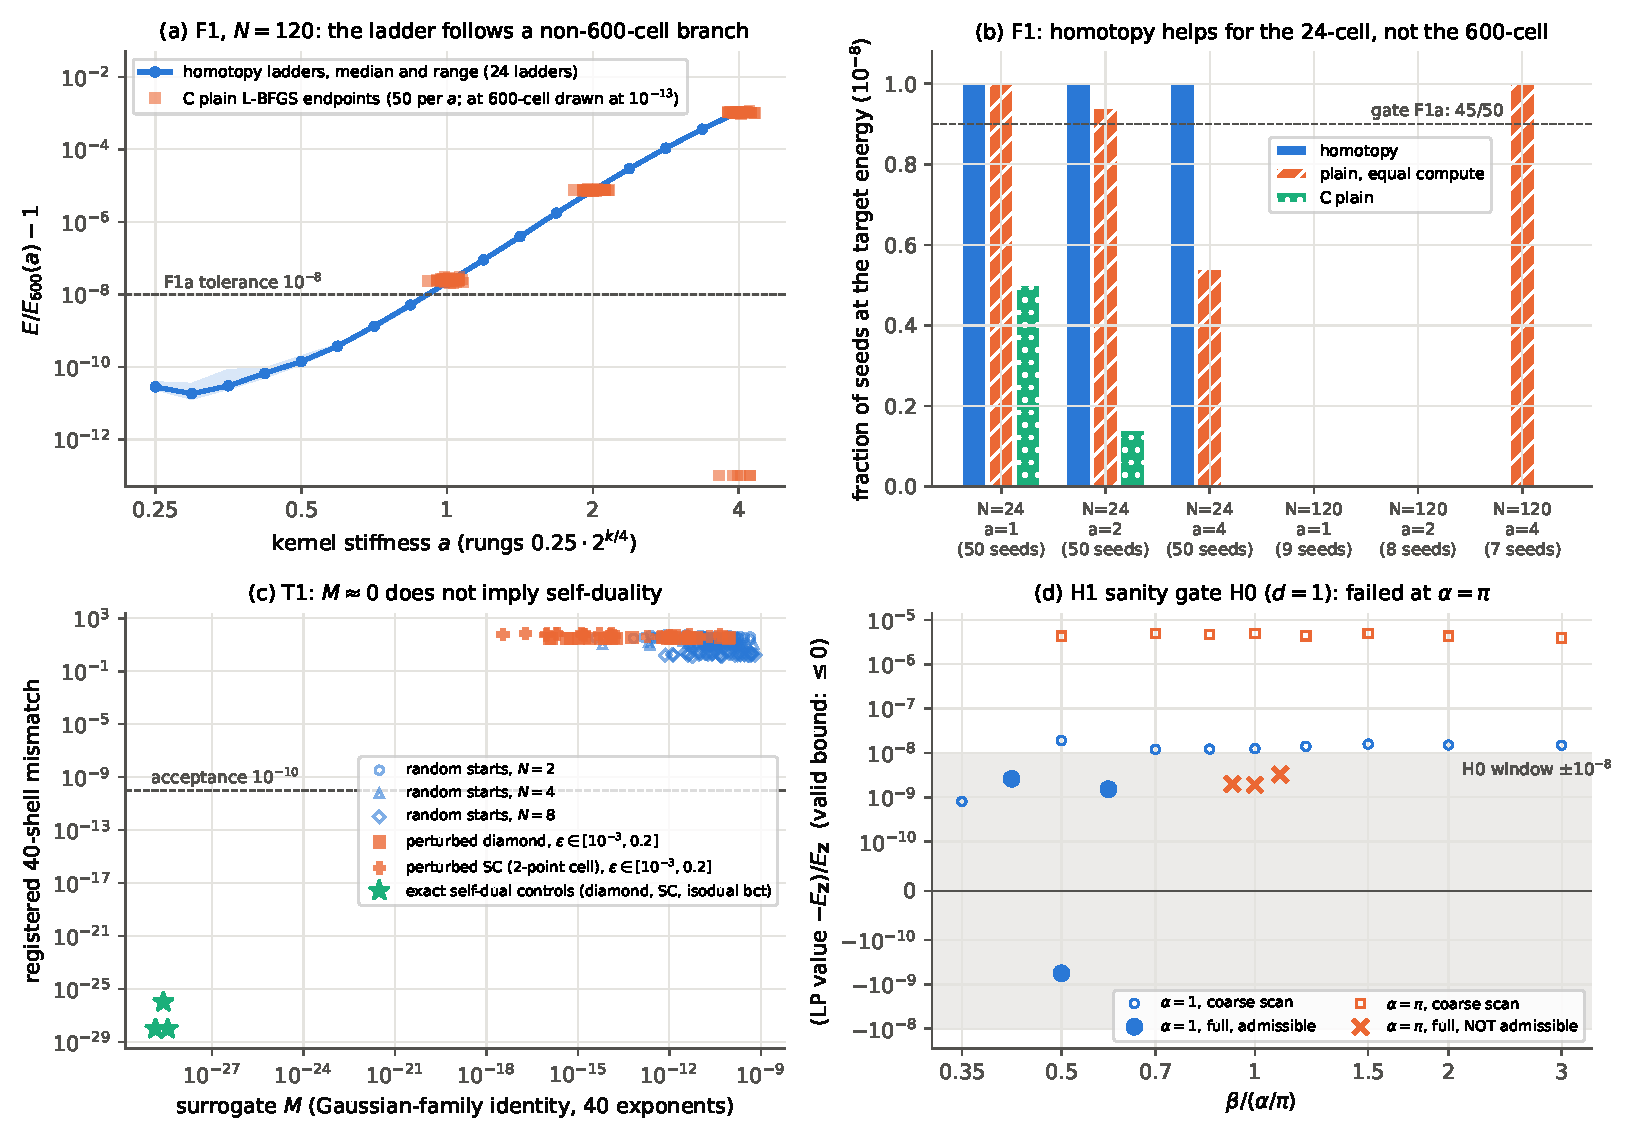
\includegraphics[width=0.98\textwidth]{figs_companion5/fig_round2.pdf}\\[2pt]
{\footnotesize Round~2. (a) F1, $N=120$: relative energy above the 600-cell along the $\alpha$-ladders (line: median; band: range)
and C's plain endpoints at $a=1,2,4$ (squares; runs that reach the 600-cell are drawn at $10^{-13}$). (b) Fraction of seeds reaching
the target energy: homotopy, plain L-BFGS with restarts at equal compute, and C's plain runs at the same seeds. (c) T1: surrogate
value against the registered shell mismatch for random starts, perturbed positive controls and the exact controls. (d) H1 sanity
gate in $d=1$: LP value minus $E_{\mathbb Z}$ (a valid bound is $\le0$) over the $\beta$ scan; crosses are full-setting solutions
that miss the admissibility tolerance.}
\end{center}
\subsection{F1: homotopy in $\alpha$ against the proved control}
Same $N=120$ points on $S^3$ and kernels $e^{-ad^2}$ as in C; from C's random start at the same seed, L-BFGS to convergence at
$a_0=0.25$, then a geometric ladder of ratio $2^{1/4}$ to the target (rungs 8, 12, 16 for $a=1,2,4$), warm-started and with C's
optimiser settings. Gate F1a: $\ge45/50$ seeds within $10^{-8}$ (relative) of $E_{600}$ \emph{and} minimum chord within $10^{-6}$ of
$2\sin(\pi/10)$. Gate F1b: plain L-BFGS from the same start with restarts, hard-capped at the homotopy's number of gradient
evaluations ($\approx7$--$9.5\times10^4$), must \emph{not} also reach $\ge45/50$ at $a\in\{2,4\}$.
\begin{center}\small
\begin{tabular}{lccccc}\toprule
$a$ & homotopy at 600-cell & plain, equal compute & C plain (same seeds) & homotopy end, rel.\ excess & gradient evaluations\\\midrule
1 & F1H1 & F1P1 & F1C1 & F1X1 & F1N1\\
2 & F1H2 & F1P2 & F1C2 & F1X2 & F1N2\\
4 & F1H4 & F1P4 & F1C4 & F1X4 & F1N4\\\bottomrule
\end{tabular}
\end{center}
\textbf{F1a fails at every $a$.} The rung-by-rung record locates the failure: already at $a_0=0.25$ the converged state is
$3\times10^{-11}$ above $E_{600}$ and yet is not the 600-cell (one ladder re-run with chords recorded, \texttt{F1/supp\_rung\_chords.py}, seed 0: converged, minimum chord $0.237$ against $0.618$, distance-spectrum deviation $0.38$), and the excess then grows smoothly along the ladder
($2\times10^{-8}$ at $a=1$, $7\times10^{-6}$ at $a=2$, $10^{-3}$ at $a=4$) --- the same excesses as C's trapped plain runs. The soft
kernel does not select the 600-cell; it selects a family of nearby minima that the ladder then follows. Seven to nine of the 17
rungs stop at C's 8\,000-iteration cap, so the soft rungs are not fully converged; the registered settings were kept. At $a=4$
plain L-BFGS \emph{with restarts} at equal compute finds the 600-cell in F1P4 seeds: the per-run success rate of fresh restarts is
F1RATE (completed runs only; the budget-truncated last run of each seed is dropped, a small survivorship bias), against 6/50
in C. A separate unregistered check with 40 fresh seeds (\texttt{F1/fresh\_plain\_a4.py}) gives F1FRESH. F1PTEST; F1CREPRO.

Control $N=24$ (50 seeds): the homotopy ends at the 24-cell energy in 50/50 starts at every $a$ (44/50 also match the chord at
$a=1$, where six end at the 24-cell energy to $10^{-8}$ with a minimum chord $1$--$2\times10^{-6}$ from 1, just outside the
$10^{-6}$ tolerance --- incomplete convergence, not a different configuration), against C's plain 25, 7, 0 of 50 and plain
with restarts at equal compute 50, 47, 27 of 50; it never goes below the 24-cell. So the homotopy \emph{does} help at $N=24$, a
configuration known not to be universally optimal, and does not at $N=120$, where the target is proved.

\textbf{Consequence (registered stop rule).} F1a failed at every $a$; the three-dimensional structure searches of this programme
(B, T2, T1) are declared unreliable, and their negatives are read only as ``no counterexample found with an unreliable search''.

\subsection{T2: Gaussian mixtures across the self-dual point}
Kernel $e^{-a_1r^2}+\lambda e^{-a_2r^2}$, $(a_1,a_2)\in\{(\pi/2,2\pi),(\pi/4,4\pi),(2,5)\}$; $\lambda^*$ (where $E_{\rm FCC}=E_{\rm BCC}$)
by bisection to $10^{-12}$, then $\lambda\in\lambda^*\{0.9,0.97,1,1.03,1.1\}$; Experiment B's engine unchanged except for an appended
mixture class (bit-identical on the stored references). For $a_1a_2=\pi^2$ the mixture with $\lambda=(\pi/a_1)^{3/2}$ is exactly
self-dual ($\hat f=f$); the bisection recovers $\lambda^*=2\sqrt2$ (to $1.9\times10^{-12}$) and $8$ (to $2.3\times10^{-10}$; the
limit is double-precision cancellation, since the FCC--BCC difference of the $a_2=4\pi$ term is only $4.8\times10^{-7}$ against
energies of order 3.5). Search: $N\in\{2,4,8,12,16\}$ with round~1's restart counts, 5\,100 restarts in
75 cells. \textbf{Gate T2: 0 candidates}; no cell has anything below the best reference lattice (most negative
relative difference $-1.9\times10^{-15}$, i.e.\ ties), and in 14 cells (pair $(\pi/4,4\pi)$, $N\ge8$) the lowest energy found is
above it by up to $3.7\times10^{-13}$ relative. The FCC/BCC crossover of the mixture kernels, including the two exactly self-dual ones, is crossed without
any intermediate non-lattice structure for $N\le16$. Hit fractions are 0.75--1.00 at $\lambda^*$ (FCC and BCC are then one
target) and 0.33--0.72 elsewhere, as in round~1. Remark: a fixed-density cell with $N\le16$ is not expected to represent the two-density
coexistence that CKS list as the lowest known energy at $\alpha=\pi$ ($4\times10^{-6}$ below the pure lattices; our engine's $E_{\rm FCC}(\pi)$ is
$4.1\times10^{-6}$ above their coexistence energy, consistent), so T2 says nothing about coexistence.

\subsection{T1: formally self-dual configurations at $\alpha=\pi$}
Definition as implemented (radial form of~\cite{CKS09}, Sec.~VI, at density 1, $Q=P$): the pair-difference measure of $P$ (weights
$1/N$) equals its structure-factor measure on $\Lambda^*$ (weights $|S(w)|^2/N^2$; the pre-registration wrote $|S|^2/N$, the
Poisson-consistent normalisation is $N^2$). Detector: the first 40 non-zero shells of each side, mismatch $<10^{-10}$. Controls
before any search: diamond $1\times10^{-26}$ (positive), FCC$\leftrightarrow$BCC $0$, $\mathbb Z^3$ $0$, the isodual bct
$9\times10^{-30}$, HCP $3\times10^3$ and FCC with itself $3.5\times10^4$ (negative). Search: a smooth surrogate (the identity tested
on 40 Gaussians, exponents 0.94--10.5, relative residuals) minimised from 60, 60, 40 random starts for $N=2,4,8$, acceptance by
the registered detector. \textbf{0 accepted} (minimum mismatch 19.8, 7.7, 1.26; a polish stage minimising the shell residuals directly lowered
the $N=8$ minimum to 0.30). The grouping tolerance ($10^{-6}$) and weight floor ($10^{-8}$) of the detector are implementation
choices, not registered.

\begin{failbox}
\textbf{Why the T1 negative is uninformative} (diagnostics added after the run, unregistered). (i) The best records have surrogate
$\sim10^{-15}$ while their pair and structure-factor measures visibly differ (L1 distance of the cumulative distributions 0.7--2.4,
0 for diamond). The identity is analytic in $\alpha$, so exact vanishing on an interval would force equality; what fails is
numerical: 40 sampled exponents with relative residuals $\sim10^{-8}$ admit configurations whose measures differ at $O(1)$ (the
best $N=2$ record has relative residual $1.2\times10^{-10}$ at $\alpha=0.3$ but $3\times10^{-3}$ at $\alpha=30$) --- the
problem is ill-conditioned. (ii) From diamond and from $\mathbb Z^3$ written as a 2-point cell, perturbed by $10^{-3}$--$0.2$, the
minimiser ends at surrogate $\le10^{-10}$ in 50/50 cases and is accepted in \textbf{0/50}. At $\varepsilon=10^{-3}$ the
\emph{unminimised} perturbed diamond already has surrogate $3.6\times10^{-11}$ (shell mismatch 30.5): the surrogate cannot resolve a
$10^{-3}$ displacement from the known solution, so the minimiser has nothing to return along. (iii) The detector is exact on the
controls but discontinuous: under perturbation diamond's systematically absent reflections reappear in the structure-factor
measure with weights $<5\times10^{-5}$ (above the $10^{-8}$ floor), have no counterpart in the pair measure, and shift the
shell-by-shell comparison (mismatch $\sim30$). The end states are nevertheless genuinely not self-dual (relative residual
$1.5\times10^{-5}$ at $\alpha=30$, CDF distance 0.022 for the $\varepsilon=10^{-3}$ case). T1 therefore reports a method
failure, not an absence of formally self-dual configurations below FCC/BCC. A usable version needs an identifying objective or an
algebraic enumeration of the CKS constructions.
\end{failbox}

\subsection{H1: the two-point LP gap}
Cohn--Kumar bound~\cite{CK07} in the periodic form $E_g(P)\ge\hat f(0)-f(0)$ for radial $f\le g$ off the origin with $\hat f\ge0$ (the registered transcription from~\cite{CK07} was not made; the statement
was derived and its proof checked, \texttt{H1/RESULTS.md}, a deviation); ansatz $\hat f(y)=e^{-\pi|y|^2/\beta}p(|y|^2)$, $\deg p\le30$, in the Laguerre eigenbasis
of the Fourier transform; HiGHS LP with cutting planes, 40-digit tail certificates, and an admissibility tolerance (polished violation
$\le5\times10^{-9}$) fixed in code before the run --- on file timestamps, not a commit --- and not in the pre-registration. Sanity gate H0 in $d=1$, where $\mathbb Z$ is universally optimal and the bound is sharp:
at $\alpha=1$ the bound is $0.7726372068$ against $E_{\mathbb Z}=0.7726372048$ ($+2\times10^{-9}$, inside the registered $10^{-8}$,
and also a measure of the discretisation error, since a valid bound cannot exceed $E_{\mathbb Z}$); at $\alpha=\pi$ the
full-setting values are $+1.6$ to $+2.8\times10^{-10}$ from $E_{\mathbb Z}$, inside the registered $10^{-8}$, but none meets the
code's admissibility tolerance (violations $2$--$5\times10^{-8}$). \textbf{H0 failed under the code's admissibility tolerance
(not registered); the stop then followed the registered rule}, and the $d=3$ gap has no value in this paper. The registered
$10^{-8}$ and the code's $5\times10^{-9}$ measure the same discretisation error from two sides (the $\alpha=1$ value is itself
$2\times10^{-9}$ \emph{above} $E_{\mathbb Z}$); part of the failure may also be a limit of the $K=30$ ansatz rather than of
certification. The H1
thresholds ($10^{-6}$, $10^{-3}$) lie far above this $10^{-8}$ level, so a re-registered run with exact (rational or
sum-of-squares) non-negativity certificates would probably be informative; it is left open.

\subsection{Round 2 deviations}
F1: the run was interrupted after 6 of 50 seeds when the launching session was compacted and resumed for seeds 6--49 with the
same code and single-threaded BLAS; \texttt{run\_F1.py} replaces C's energy evaluator by an equivalent
Gram-matrix form, asserted equal to $10^{-12}$ before every run (an oversubscribed first resume was stopped after 8 minutes, before any record). By then F1a
had already failed at every $a$ (6 misses each, more than the 5 allowed). The N$=24$ control completed in the first session.
T2: mixture class appended; diamond and A15 added for information. T1: the $N^2$ normalisation; surrogate run~1 (16 Gaussians,
absolute residuals) uninformative and discarded with records kept; run~2 start counts not registered (60/60/40); a typo in the
bct control fixed and rerun; an earlier draft and stale code comments in \texttt{expT1.py} and \texttt{selfdual.py}
misdescribed run~2's surrogate, corrected after a partial rerun reproduced 20 run-2 records bit for bit; detector tolerances not
registered. H1: the admissibility tolerance was fixed in code before the run but not in the
pre-registration (file timestamps only); \texttt{lp\_bound.py} was touched during the run, a docstring-only change (compiled
bytecode identical); tail grids and certificates added; the bound was derived rather than transcribed. All four were written up after a context compaction of the session that
launched them, from the records and logs only.
